\section{Data}
\label{sec:Data}

\subsection{DDSM}
\label{subsec: Date_DDSM}

Most computer-aided diagnosis (CADx) and 
detection (CADe) algorithms for breast cancer 
in mammography are evaluated on private data 
sets or on unspecified subsets of public 
databases. 
\cite{Gao2019}
This causes an inability to 
directly compare the performance of methods or 
to replicate prior results. 
\cite{Choukroun2017}
To resolve this substantial challenge by releasing 
an updated and standardized version of the 
Digital Database for Screening Mammography 
(DDSM) for evaluation of future CADx and CADe 
systems (sometimes referred to generally as CAD) 
research in mammography.
\cite{Zhu2017}
The CBIS-DDSM (Curated Breast Imaging Subset of 
DDSM), includes decompressed images, data 
selection, curation by trained mammographers, 
updated mass segmentation, bounding 
boxes, and pathologic diagnosis for training 
data, formatted similarly to modern computer 
vision data sets. The data set contains 753 
calcification cases and 891 mass cases, 
providing a data-set size capable of 
analyzing decision support systems in 
mammography. As shown in Figure~\ref{fig:figData}

\begin{figure*}[!ht]
    \centering
    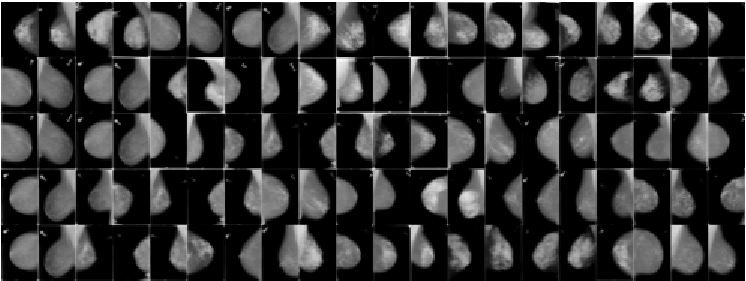
\includegraphics[
        width=1.0\textwidth,
        keepaspectratio
        ]{Data.pdf}
    \caption{Examples in the dataset}
    \label{fig:figData}
\end{figure*}

\subsection{Augmentation}
\label{subsec: Date_Aug}

Compared to other common data sets 
(e.g. Pascal Voc) in the field of image 
object detection, the DDSM data set 
is relatively small. 
\cite{M.HeathK.BowyerD.Kopans2001}
Since small data 
sets are prone to reduce the model effect, 
to maintain the representation power of 
model and avoid overfitting in some ways, 
several data augmentation methods are 
employed. We don’t augment data with the
crop, translate or scale operations to 
avoid changing the original label of images.
Instead, we randomly rotate and shear the 
original images between -10$^{\circ}$ and 
10$^{\circ}$ , then flip them horizontally 
or vertically and fill the margin with 
white pixels. 